\documentclass[]{beamer}
\usepackage[T1]{fontenc}
\usepackage[utf8]{inputenc}
\usepackage{lmodern}
\usepackage[italian]{babel}

\title{Il primo principio della termodinamica}
\author{\texorpdfstring{Mattia Cozzi\newline\href{mailto:cozzimattia@gmail.com}{\texttt{cozzimattia@gmail.com}}}{Mattia Cozzi}}
\date{a.s.~2023/2024}

%\documentclass[handout]{beamer}     %usare questa classe per generare l'handout
%\usepackage{pgfpages}   %per mostrare più quadri nella stessa pagina
%\pgfpagesuselayout{4 on 1}[a4paper,border shrink=5mm,landscape]
\usetheme{Singapore}
%\useoutertheme[left]{sidebar} %elementi intorno alle diapositive
\setbeamercovered{dynamic} %modifica l'aspetto del testo grigetto delle diapositive future. Argomenti: invisible/transparent/dynamic
\usecolortheme{orchid}
%COLORE PRINCIPALE
% \definecolor{marroncino}{RGB}{156, 26, 0} % UBC Blue (primary)
% \setbeamercolor{structure}{fg=marroncino} % itemize, enumerate, etc

\theoremstyle{plain}
\newtheorem{teorema}{Teorema}

\usepackage{tikz}


\usepackage{pgf,pgfplots,graphicx}
\usetikzlibrary{angles,quotes,arrows,shapes,decorations.markings}
\pgfplotsset{compat=1.15}
\usepgfplotslibrary{units,fillbetween} % to add units easily to axis
\tikzset{fleche/.style args={#1:#2}{postaction=decorate,decoration={name=markings,mark=at position #1 with {\arrow[#2,scale=2]{>}}},},}



\begin{document}

\begin{frame}
  \titlepage
\end{frame}





\begin{frame}
\frametitle{Contenuti}
\tableofcontents
\end{frame}

\section{Sistema e ambiente}

\begin{frame}
\frametitle{Contesto storico}
\begin{columns}
\begin{column}{0.2\textwidth}
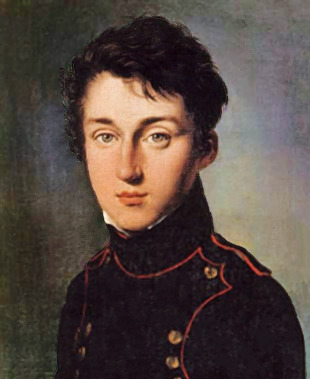
\includegraphics[width=\columnwidth]{img/carnot.jpg}
\end{column}
\begin{column}{0.7\textwidth}
1824\\Sadi Carnot pubblica le sue \emph{Riflessioni sulla potenza motrice del fuoco}, testo che contiene la sua teoria sulle macchine termiche.\pause

\begin{itemize}
\item<2-> I motori a vapore sono utilizzati su vasta scala (macchina di Watt, 1765);
\item<3-> Il principio di conservazione dell'energia non è ancora stato enunciato;
\item<4-> Non è stata dimostrata l'equivalenza tra calore e lavoro (Joule, 1847);
\item<5-> Il modello per lo studio del calore è la \emph{teoria del calorico} (un ipotetico fluido che passa da un corpo ad un altro).
\end{itemize}
\end{column}
\end{columns}
\end{frame}

\begin{frame}
\frametitle{La termodinamica}
La termodinamica:
\begin{itemize}
  \item si sviluppa nel XIX secolo, parallelamente alla rivoluzione industriale;\pause
  \item si occupa degli scambi energetici tra un \alert<2>{sistema} e l'\alert<2>{ambiente} in cui si trova.\pause
\end{itemize}

~

Gli scambi energetici possono avvenire mediante \alert<3>{calore} o \alert<3>{lavoro} (ricordarsi l'esperimento di Joule).
\end{frame}

\begin{frame}
\frametitle{Sistema e ambiente}
Definiamo:
\begin{block}{Sistema}
Porzione di spazio che viene studiata dal punto di vista degli scambi energetici.
\end{block}\pause
\begin{block}{Ambiente}
Spazio circostante il sistema, dal quale può essere separato per mezzo di un \emph{confine}.
\end{block}
\end{frame}

\begin{frame}
\frametitle{Attraversamento del confine}
Un sistema può essere:
\begin{enumerate}
  \item \alert<1>{aperto}, se il confine può essere attraversato da energia e da materia;\pause
  \item \alert<2>{chiuso}, se il confine può essere attraversato da energia ma non da materia;\pause
  \item \alert<3>{isolato}, se il confine non può essere attraversato né da materia né da energia;
\end{enumerate}
\end{frame}


\begin{frame}
\frametitle{Stato di un sistema}
Lo stato di un sistema è descritto dai suoi valori di:
\begin{itemize}
  \item pressione;
  \item volume;
  \item temperatura;
  \item numero di moli.
\end{itemize}\pause
Tali quantità sono le sue \alert<1>{variabili di stato}, legate da:
\begin{center}
$ pV = nRT $
\end{center}\pause
Un sistema è in equilibrio quando le sue variabili non cambiano nel tempo.
\end{frame}


\begin{frame}
\frametitle{Esempio}
\begin{exampleblock}{Stato di un sistema}
{\small
$ 0,20 \, mol $ di gas perfetto sono mantenute in un recipiente cilindrico mediante un pistone mobile, a tenuta e di massa trascurabile. Il recipiente si trova in equilibrio con l'ambiente esterno ($ T = 20 \, ^\circ C $ e $ p = 1,0 \, atm $) quando il pistone si posiziona a $ 50 \, cm $ d'altezza rispetto al fondo del recipiente.

Determina il raggio del pistone.}
\end{exampleblock}
\end{frame}

\begin{frame}
\frametitle{Energia interna}
Abbiamo capito che la temperatura di un gas dipende dall'agitazione termica delle sue particelle, che possiedono quindi una certa energia.\pause

~

Tale energia è l'energia interna $ U $ del sistema e vale:
\begin{columns}
\begin{column}{0.4\textwidth}
\begin{center}
$ U = \dfrac{3}{2}nRT $

\vspace*{.7em}
per gas monoatomici
\end{center}
\end{column}
\begin{column}{0.4\textwidth}
\begin{center}
$ U = \dfrac{5}{2}nRT $

\vspace*{.7em}
per gas biatomici
\end{center}
\end{column}
\end{columns}\pause

~

~

Vediamo come $ U $ dipenda dallo stato del sistema. Viene detta pertanto \alert{funzione di stato}, che dipende dalle variabili di stato del sistema.
\end{frame}



\begin{frame}
\frametitle{Esempio}
\begin{exampleblock}{Variazione di energia interna}
{\small Una mole di gas perfetto monoatomico passa da una temperatura $ 270 \, K $ ad una temperatura di $ 350 \, K $.

Calcola la sua variazione di energia interna.}
\end{exampleblock}
\end{frame}




\section{Primo principio}

\begin{frame}
\frametitle{Sistema modello}
Per studiare i sistemi termodinamici introduciamone un \emph{modello semplificato}.

\begin{columns}
\begin{column}{0.5\textwidth}
\begin{figure}
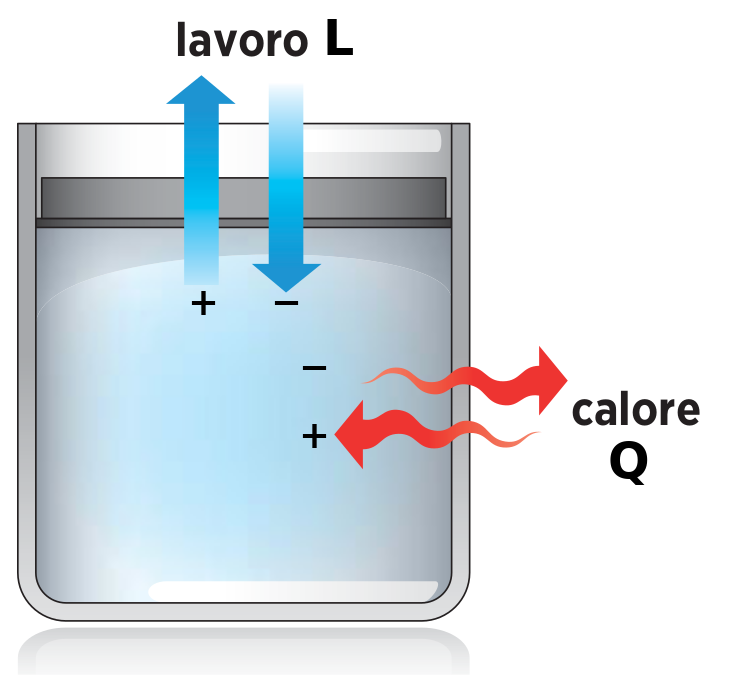
\includegraphics[width=\columnwidth]{img/sistemamodello0.png}
\end{figure}
\end{column}
\begin{column}{0.4\textwidth}
Cilindro chiuso, pieno di gas perfetto, con un pistone mobile. \alert<1>{Può scambiare calore e lavoro con l'ambiente}.\pause

~

\alert<2>{Attenzione alle convenzioni sui segni!}
\end{column}
\end{columns}
\end{frame}

\begin{frame}
\frametitle{Segno delle quantità}
Il lavoro $ L $:
\begin{itemize}
  \item è positivo se il pistone sale (il sistema fa lavoro sull'ambiente);\pause
  \item è negativo se il pistone scende (il sistema subisce un lavoro dall'ambiente).\pause
\end{itemize}

~

Il calore $ Q $:
\begin{itemize}
  \item è positivo se viene ricevuto dal sistema;\pause
  \item è negativo se viene perso dal sistema.
\end{itemize}
\end{frame}


\begin{frame}
\frametitle{Enunciato del primo principio}
\begin{block}{Primo principio della termodinamica}
\begin{center}
\colorbox{blue!30}{$ \Delta U = Q - L $}
\end{center}
La variazione di energia interna del sistema è uguale all'energia scambiata con l'ambiente (sotto forma di calore o di lavoro).
\end{block}\pause

~

È uno dei modi in cui possiamo esprimere il \alert{principio di conservazione dell'energia}.
\end{frame}



\begin{frame}
\frametitle{Esempi}
\begin{exampleblock}{Utilizzo del primo principio}
{\small $ 1,50 \, mol $ di gas perfetto monoatomico passano da  $ 300 \, K $ a $ 600 \, K $ quando ricevono $ 8,00 \times 10^4 \, J $ di calore.

Calcola il lavoro compiuto dal gas.}
\end{exampleblock}

~

\begin{exampleblock}{Lavoro e calore}
{\small Dimostra che durante una trasformazione isoterma il lavoro compiuto dal gas è uguale al calore ricevuto.}
\end{exampleblock}
\end{frame}






\section{Trasformazioni}

\begin{frame}
\frametitle{Trasformazioni termodinamiche}
Si ha una trasformazione termodinamica quando un sistema passa da uno stato A ad uno stato B.

~

Una trasformazione può essere:
\begin{itemize}
  \item \alert<1>{ideale}, se ogni stato intermedio è uno stato di equilibrio;\pause
  \item \alert<2>{reale}, se il sistema non passa uniformemente da uno stato di equilibrio all'altro.\pause 
\end{itemize}

~

Una trasformazione molto lenta è una buona approssimazione di una trasformazione ideale.

Sono dette \alert{trasformazioni quasi-statiche}.
\end{frame}

\begin{frame}
\frametitle{Trasformazioni reversibili}
Le trasformazioni ideali possono essere percorse esattamente a ritroso e sono pertanto reversibili.\pause

~

\begin{block}{Trasformazione reversibile}
Una trasformazione è reversibile se è possibile riportare sia il sistema sia l'ambiente allo stato iniziale.
\end{block}\pause

~

Una trasformazione reale non è mai perfettamente reversibile.
\end{frame}



\begin{frame}
\frametitle{Piano di Clapeyron}
Le trasformazioni termodinamiche vengono rappresentate su un piano volume/pressione.\pause

~

\begin{columns}
\begin{column}{0.4\textwidth}
\begin{figure}
\begin{tikzpicture}[scale=0.45]
\begin{axis}[
axis x line=bottom,
axis y line=left,
xmin=0, xmax=5,
ymin=0, ymax=4,
xlabel={$V\, [m^3] $},
x label style={at={(axis cs:5,0)},anchor=north},
ylabel={$p\, [Pa] $},
y label style={at={(axis cs:0,4)},rotate=0,anchor=south},
xtick={},
xticklabels={,,},
ytick={},
yticklabels={,,},
]
\node [below,red] at (1,1) {$ A $};
\node [above,red] at (4,3) {$ B $};
        \draw [
            fleche={0.5:red},
            thick,red              % <-- added
        ] (axis cs:1,1) to [bend right=30]
            % store start and end coordinates
            coordinate [pos=0] (start)
            coordinate [pos=1] (end)
        (axis cs:4,3);

        % draw start and end point
        \fill [radius=2pt,red]
            (start) circle[]
            (end)   circle[];
    \end{axis}
\end{tikzpicture}
\end{figure}
\end{column}
\begin{column}{0.4\textwidth}
\begin{figure}
\begin{tikzpicture}[scale=0.45]
\begin{axis}[
axis x line=bottom,
axis y line=left,
xmin=0, xmax=5,
ymin=0, ymax=4,
xlabel={$V\, [m^3] $},
x label style={at={(axis cs:5,0)},anchor=north},
ylabel={$p\, [Pa] $},
y label style={at={(axis cs:0,4)},rotate=0,anchor=south},
xtick={},
xticklabels={},
ytick={},
yticklabels={},
]
\node [below,red] at (4,1) {$ A $};
\node [above,red] at (1,3.6) {$ B $};
        % now draw the curve
        \draw [
            fleche={0.66:red},
            thick,red              % <-- added
        ] (axis cs:1,3.6) to [bend right=20]
            % store start and end coordinates
            coordinate [pos=0] (start)
            coordinate [pos=1] (end)
        (axis cs:4,1);
        % now draw the curve
        \draw [
            fleche={0.66:red},
            thick,red              % <-- added
        ] (axis cs:4,1) to [bend left=20]
            % store start and end coordinates
            coordinate [pos=0] (start)
            coordinate [pos=1] (end)
        (axis cs:1,3.6);

        % draw start and end point
        \fill [radius=2pt,red]
            (start) circle[]
            (end)   circle[];
\end{axis}
\end{tikzpicture}
\end{figure}
\end{column}
\end{columns}

~

Se la freccia è doppia, allora la trasformazione è reversibile.
\end{frame}


\begin{frame}
\frametitle{Trasformazione isobara}
Avviene a pressione costante, quando in ogni istante la pressione interna è uguale alla pressione esterna sul pistone.
\begin{figure}
\begin{tikzpicture}[scale=0.65]
\begin{axis}[
axis x line=bottom,
axis y line=left,
xmin=0, xmax=5,
ymin=0, ymax=4,
xlabel={$V\, [m^3] $},
x label style={at={(axis cs:5,0)},anchor=north},
ylabel={$p\, [Pa] $},
y label style={at={(axis cs:0,4)},rotate=0,anchor=south},
xtick={1,4},
xticklabels={$V_0$,$V_1$},
ytick={2},
yticklabels={$p_1 = p_0 $},
]

\fill [red!40,] (axis cs:1,2) |- (axis cs:4,2) |- (axis cs:1,0) --
            cycle;

        % draw the dashed lines
        % (using two different approaches)
        \addplot [dashed,domain=0:1,samples=2] {2};
        \addplot [dashed,domain=0:4,samples=2] {2};

        \draw [dashed,thin] (axis cs:4,2) -- (axis cs:4,0);
        \draw [dashed,thin] (axis cs:1,2)   -- (axis cs:1,0);
        % now draw the curve
        \draw [
            fleche={0.5:red},
            thick,red              % <-- added
        ] (axis cs:1,2) to [bend right=0]
            % store start and end coordinates
            coordinate [pos=0] (start)
            coordinate [pos=1] (end)
        (axis cs:4,2);

        % draw start and end point
        \fill [radius=2pt,red]
            (start) circle[]
            (end)   circle[];
    \end{axis}
\end{tikzpicture}
\end{figure}\pause
Per la trasformazione isobara, possiamo verificare un importante risultato.
\end{frame}


\begin{frame}
\frametitle{Lavoro in una isobara}
Sappiamo che:
\begin{center}
$ p = \dfrac{F}{S} ~~~\Longrightarrow ~~~ F = p \cdot S $
\end{center}\pause
Calcoliamo il lavoro come $ L = F \cdot s $:
\begin{center}
$ L = F \cdot \Delta h \pause = p \cdot S \cdot \Delta h \pause = p \cdot \Delta V $
\end{center}\pause

~

Il PPT avrà forma:
\begin{center}
\colorbox{blue!30}{$ \Delta U = Q - p \Delta V $}
\end{center}
\end{frame}

\begin{frame}
\frametitle{Esempio}
\begin{exampleblock}{Trasformazione isobara}
{\small 
Tre moli di gas biatomico si trovano ad una temperatura iniziale di $ 300 \, K $ e occupano un volume di $ 2,00 \times 10^{-1} \, m^3 $.

Successivamente vengono riscaldate a pressione costante e si espandono, occupando un volume pari a 5/2 di quello iniziale.

Calcola:
\begin{itemize}
    \item il valore delle temperatura finale del gas;
    \item la variazione di energia interna;
    \item il lavoro compiuto durante l'espansione;
    \item il calore fornito al gas.
\end{itemize}
}
\end{exampleblock}
\end{frame}




\begin{frame}
\frametitle{Trasformazione isocora}
Avviene a volume costante, quindi il pistone rimane fermo.
\begin{figure}
\begin{tikzpicture}[scale=0.65]
\begin{axis}[
axis x line=bottom,
axis y line=left,
xmin=0, xmax=5,
ymin=0, ymax=4,
xlabel={$V\, [m^3] $},
x label style={at={(axis cs:5,0)},anchor=north},
ylabel={$p\, [Pa] $},
y label style={at={(axis cs:0,4)},rotate=0,anchor=south},
xtick={3},
xticklabels={$V_0$},
ytick={1,3},
yticklabels={$p_0$,$p_1 $},
]


% draw the dashed lines
% (using two different approaches)
\draw [dashed,thin] (axis cs:0,1) -- (axis cs:3,1);
\draw [dashed,thin] (axis cs:0,3)   -- (axis cs:3,3);
\draw [dashed,thin] (axis cs:3,0)   -- (axis cs:3,1);

% now draw the curve
\draw [fleche={0.5:red},thick,red] 
  (axis cs:3,1) to [bend right=0]
     % store start and end coordinates
     coordinate [pos=0] (start)
     coordinate [pos=1] (end)
  (axis cs:3,3);

% draw start and end point
\fill [radius=2pt,red] (start) circle[] (end) circle[];
\end{axis}
\end{tikzpicture}
\end{figure}\pause
Poiché il pistone è fermo, il lavoro è nullo e il PPT avrà forma:
\begin{center}
\colorbox{blue!30}{$ \Delta U = Q $}
\end{center}
\end{frame}




\begin{frame}
\frametitle{Trasformazione isoterma}
Avviene a temperatura costante, quindi non può variare l'energia del sistema.
\begin{figure}
\begin{tikzpicture}[scale=0.65]
\begin{axis}[
axis x line=bottom,
axis y line=left,
xmin=0, xmax=5,
ymin=0, ymax=6,
xlabel={$V\, [m^3] $},
x label style={at={(axis cs:5,0)},anchor=north},
ylabel={$p\, [Pa] $},
y label style={at={(axis cs:0,6)},rotate=0,anchor=south},
xtick={1,3},
xticklabels={$V_0$,$V_1$},
ytick={1.5,4},
yticklabels={$p_1$,$p_0$},
]

        % fill the area below the curve
        % (draw it first, so it is below everything else)
        \fill [
            red!40,
        ]
            (axis cs:1,4) to [bend right=20]
            (axis cs:3,1.5) |-
            (axis cs:1,\pgfkeysvalueof{/pgfplots/ymin}) |-
            cycle
        ;

        % draw the dashed lines
        % (using two different approaches)
        \addplot [dashed,domain=0:1,samples=2] {4};
        \addplot [dashed,domain=0:3,samples=2] {1.5};

        \draw [dashed,thin] (axis cs:3,1.5) -- (axis cs:3,0);
        \draw [dashed,thin] (axis cs:1,4)   -- (axis cs:1,0);

        % now draw the curve
        \draw [
            fleche={0.5:red},
            thick,red              % <-- added
        ] (axis cs:1,4) to [bend right=20]
            % store start and end coordinates
            coordinate [pos=0] (start)
            coordinate [pos=1] (end)
        (axis cs:3,1.5);

        % draw start and end point
        \fill [radius=2pt,red]
            (start) circle[]
            (end)   circle[];
\end{axis}
\end{tikzpicture}
\end{figure}\pause
Se $ \Delta U = 0 $, allora $ Q - L = 0 $ e il PPT avrà forma:
\begin{center}
\colorbox{blue!30}{$ Q = L $}
\end{center}
\end{frame}


\begin{frame}
\frametitle{Trasformazione adiabatica}
Avviene senza scambio di calore con l'ambiente (il recipiente ha le pareti termicamente isolate).
\begin{figure}
\begin{tikzpicture}[,scale=0.65]
    \begin{axis}[
        axis x line=bottom,
        axis y line=left,
        xmin=0, xmax=10,
        ymin=0, ymax=10,
%        % (made labels more common)
%        % (because of the "sketch" type of the plot these should not be needed)
%        xlabel={Volume $(\mathrm{m}^3)$},
%        ylabel={Pressure (Pa)},
        % (changed ticks + labels to normal ticks instead of extra ticks)
        xtick={1,6},
        xticklabels={$V_1$,$V_2$},
        ytick={0.3,6.6},
        yticklabels={$p_2$,$p_1$},  % <-- (changed order of entries)
    ]
        % fill the area below the curve
        % (draw it first, so it is below everything else)
        \fill [
            red!40,
        ]
            (axis cs:1,6.6) to [bend right=20]
            (axis cs:6,0.3) |-
            (axis cs:6,0) |-
            (axis cs:1,\pgfkeysvalueof{/pgfplots/ymin}) --
            cycle
        ;

        % draw the dashed lines
        % (using two different approaches)

        \draw [dashed,thin] (axis cs:0,6.6) -- (axis cs:1,6.6);
        \draw [dashed,thin] (axis cs:0,0.3)   -- (axis cs:6,0.3);
        \draw [dashed,thin] (axis cs:1,0) -- (axis cs:1,6.6);
        \draw [dashed,thin] (axis cs:6,0)   -- (axis cs:6,0.3);

        \draw [
            thick,              % <-- added
            dotted,
        ] (axis cs:8,0.5) to [bend right=-30]
        (axis cs:0.5,8);
        
        \draw [
            thick,              % <-- added
            dotted,
        ] (axis cs:7,0.2) to [bend right=-40]
        (axis cs:0.2,7);

        \draw [
            fleche={0.6:red},
            thick,red              % <-- added
        ] (axis cs:1,6.6) to [bend right=20]
            % store start and end coordinates
            coordinate [pos=0] (start)
            coordinate [pos=1] (end)
        (axis cs:6,0.3);
        

        % draw start and end point
        \fill [radius=2pt,red]
            (start) circle[]
            (end)   circle[];
    \end{axis}
\end{tikzpicture}
\end{figure}\pause
Senza scambio di calore $ Q = 0 $ e il PPT avrà forma:
\begin{center}
\colorbox{blue!30}{$ \Delta U = - L $}
\end{center}
\end{frame}



\begin{frame}
\frametitle{Trasformazione ciclica}
In una ciclica si parte da uno stato per poi ritornarci.
\begin{figure}
\begin{tikzpicture}[,scale=0.65]
    \begin{axis}[
        axis x line=bottom,
        axis y line=left,
        xmin=0, xmax=10,
        ymin=0, ymax=10,
%        % (made labels more common)
%        % (because of the "sketch" type of the plot these should not be needed)
%        xlabel={Volume $(\mathrm{m}^3)$},
%        ylabel={Pressure (Pa)},
        % (changed ticks + labels to normal ticks instead of extra ticks)
        xtick={3,6},
        xticklabels={$V_1$,$V_2$},
        ytick={1.5,6},
        yticklabels={$p_2$,$p_1$},  % <-- (changed order of entries)
    ]
        % fill the area below the curve
        % (draw it first, so it is below everything else)
%         \fill [
%             red!40,
%         ]
%             (axis cs:3,6) to [bend right=30]
%             (axis cs:6,1.5) |-
%             (axis cs:3,\pgfkeysvalueof{/pgfplots/ymin}) --
%             cycle
%         ;
        \fill [
            red!40,
        ]
            (axis cs:6,1.5) to [bend right=60]
            (axis cs:3,6) to [bend right= 60]
            cycle
        ;

        % draw the dashed lines
        % (using two different approaches)
        \addplot [dashed,domain=0:3,samples=2] {6};
        \addplot [dashed,domain=0:6,samples=2] {1.5};

        \draw [dashed,thin] (axis cs:6,1.5) -- (axis cs:6,0);
        \draw [dashed,thin] (axis cs:3,6)   -- (axis cs:3,0);

        % now draw the curve
        \draw [
            fleche={0.6:red},
            thick,red              % <-- added
        ] (axis cs:3,6) to [bend right=60]
            % store start and end coordinates
            coordinate [pos=0] (start)
            coordinate [pos=1] (end)
        (axis cs:6,1.5);

        \draw [
            fleche={0.6:red},
            thick,red              % <-- added
        ] (axis cs:6,1.5) to [bend right=60]
            % store start and end coordinates
            coordinate [pos=0] (start)
            coordinate [pos=1] (end)
        (axis cs:3,6);

        % draw start and end point
        \fill [radius=2pt,red]
            (start) circle[]
            (end)   circle[];
    \end{axis}
\end{tikzpicture}
\end{figure}\pause
Se si torna allo stato iniziale, $ \Delta U = 0 $ e il PPT avrà forma:
\begin{center}
\colorbox{blue!30}{$ Q = L $}
\end{center}
\end{frame}


\section{Lavoro}

\begin{frame}
\frametitle{Lavoro termodinamico (1)}
Il lavoro svolto dal sistema durante una trasformazione dipende dalla trasformazione stessa, cioè dallo specifico percorso seguito.\pause

~

Il lavoro pertanto \alert<2>{non è una funzione di stato}.\pause
\begin{columns}
\begin{column}{0.4\textwidth}
\begin{figure}
\begin{tikzpicture}[scale=0.55]
\begin{axis}[
axis x line=bottom,
axis y line=left,
xmin=0, xmax=5,
ymin=0, ymax=4,
xlabel={$V\, [m^3] $},
x label style={at={(axis cs:5,0)},anchor=north},
ylabel={$p\, [Pa] $},
y label style={at={(axis cs:0,4)},rotate=0,anchor=south},
xtick={1,4},
xticklabels={$V_0$,$V_1$},
ytick={2},
yticklabels={$ p $},
]

\fill [red!40,] (axis cs:1,2) |- (axis cs:4,2) |- (axis cs:1,0) --
            cycle;

        % draw the dashed lines
        % (using two different approaches)
        \addplot [dashed,domain=0:1,samples=2] {2};
        \addplot [dashed,domain=0:4,samples=2] {2};

        \draw [dashed,thin] (axis cs:4,2) -- (axis cs:4,0);
        \draw [dashed,thin] (axis cs:1,2)   -- (axis cs:1,0);
        % now draw the curve
        \draw [
            fleche={0.5:red},
            thick,red              % <-- added
        ] (axis cs:1,2) to [bend right=0]
            % store start and end coordinates
            coordinate [pos=0] (start)
            coordinate [pos=1] (end)
        (axis cs:4,2);

        % draw start and end point
        \fill [radius=2pt,red]
            (start) circle[]
            (end)   circle[];
        \node [below,red] at (2.5,1.3) {{\huge $ L $}};
    \end{axis}
\end{tikzpicture}
\end{figure}
\end{column}
\begin{column}{0.45\textwidth}
Per le isobare vale $ L = p \Delta V $, che risulta essere l'area del rettangolo in figura.\pause

~

In generale, il lavoro durante una trasformazione è l'\alert{area sottesa dalla curva} che la rappresenta.
\end{column}
\end{columns}
\end{frame}






\begin{frame}
\frametitle{Lavoro termodinamico (2)}
\begin{columns}
\begin{column}{0.4\textwidth}
\begin{figure}
\begin{tikzpicture}[scale=0.55]
\begin{axis}[
axis x line=bottom,
axis y line=left,
xmin=0, xmax=5,
ymin=0, ymax=6,
xlabel={$V\, [m^3] $},
x label style={at={(axis cs:5,0)},anchor=north},
ylabel={$p\, [Pa] $},
y label style={at={(axis cs:0,6)},rotate=0,anchor=south},
xtick={},
xticklabels={},
ytick={},
yticklabels={},
]

        % fill the area below the curve
        % (draw it first, so it is below everything else)
        \fill [
            red!40,
        ]
            (axis cs:1,4) to [bend right=20]
            (axis cs:3,1.5) |-
            (axis cs:1,\pgfkeysvalueof{/pgfplots/ymin}) |-
            cycle
        ;

        % now draw the curve
        \draw [
            fleche={0.5:red},
            thick,red              % <-- added
        ] (axis cs:1,4) to [bend right=20]
            % store start and end coordinates
            coordinate [pos=0] (start)
            coordinate [pos=1] (end)
        (axis cs:3,1.5);

        % draw start and end point
        \fill [radius=2pt,red]
            (start) circle[]
            (end)   circle[];
        \node [below,red] at (2,1.3) {{\huge $ L >0 $}};
\end{axis}
\end{tikzpicture}
\end{figure}
\end{column}
\begin{column}{0.4\textwidth}
\begin{figure}
\begin{tikzpicture}[scale=0.55]
\begin{axis}[
axis x line=bottom,
axis y line=left,
xmin=0, xmax=5,
ymin=0, ymax=6,
xlabel={$V\, [m^3] $},
x label style={at={(axis cs:5,0)},anchor=north},
ylabel={$p\, [Pa] $},
y label style={at={(axis cs:0,6)},rotate=0,anchor=south},
xtick={},
xticklabels={},
ytick={},
yticklabels={},
]

        % fill the area below the curve
        % (draw it first, so it is below everything else)
        \fill [
            blue!40,
        ]
            (axis cs:3,1.5) to [bend right=20]
            (axis cs:1,4) |-
            (axis cs:3,0) |-
            cycle
        ;

        % now draw the curve
        \draw [
            fleche={0.5:blue},
            thick,blue              % <-- added 
        ] (axis cs:3,1.5) to [bend right=20]
            % store start and end coordinates
            coordinate [pos=0] (start)
            coordinate [pos=1] (end)
        (axis cs:1,4);

        % draw start and end point
        \fill [radius=2pt,blue]
            (start) circle[]
            (end)   circle[];
        \node [below,blue] at (2,1.3) {{\huge $ L < 0 $}};
\end{axis}
\end{tikzpicture}
\end{figure}
\end{column}
\end{columns}

~

Se il volume aumenta avremo lavoro positivo, se invece il volume diminuisce avremo lavoro negativo.
\end{frame}

\begin{frame}
\frametitle{Lavoro termodinamico (3)}
\begin{columns}
\begin{column}{0.4\textwidth}

\begin{figure}
\begin{tikzpicture}[scale=0.45]
\begin{axis}[
axis x line=bottom,
axis y line=left,
xmin=0, xmax=5,
ymin=0, ymax=6,
xlabel={$V\, [m^3] $},
x label style={at={(axis cs:5,0)},anchor=north},
ylabel={$p\, [Pa] $},
y label style={at={(axis cs:0,6)},rotate=0,anchor=south},
xtick={},
xticklabels={},
ytick={},
yticklabels={},
]

        % fill the area below the curve
        % (draw it first, so it is below everything else)
        \fill [
            red!40,
        ]
            (axis cs:1,4) to [bend left=40]
            (axis cs:3,1.5) |-
            (axis cs:1,\pgfkeysvalueof{/pgfplots/ymin}) |-
            cycle
        ;

        % now draw the curve
        \draw [
            fleche={0.5:red},
            thick,red              % <-- added
        ] (axis cs:1,4) to [bend left=40]
            % store start and end coordinates
            coordinate [pos=0] (start)
            coordinate [pos=1] (end)
        (axis cs:3,1.5);

        % draw start and end point
        \fill [radius=2pt,red]
            (start) circle[]
            (end)   circle[];
        \node [below,red] at (2,1.3) {{\huge $ L_1 > 0 $}};
\end{axis}
\end{tikzpicture}
\end{figure}
\end{column}
\begin{column}{0.4\textwidth}
\begin{figure}
\begin{tikzpicture}[scale=0.45]
\begin{axis}[
axis x line=bottom,
axis y line=left,
xmin=0, xmax=5,
ymin=0, ymax=6,
xlabel={$V\, [m^3] $},
x label style={at={(axis cs:5,0)},anchor=north},
ylabel={$p\, [Pa] $},
y label style={at={(axis cs:0,6)},rotate=0,anchor=south},
xtick={},
xticklabels={},
ytick={},
yticklabels={},
]

        % fill the area below the curve
        % (draw it first, so it is below everything else)
        \fill [
            blue!40,
        ]
            (axis cs:3,1.5) to [bend left=40]
            (axis cs:1,4) |-
            (axis cs:3,0) |-
            cycle
        ;

        % now draw the curve
        \draw [
            fleche={0.5:blue},
            thick,blue              % <-- added 
        ] (axis cs:3,1.5) to [bend left=40]
            % store start and end coordinates
            coordinate [pos=0] (start)
            coordinate [pos=1] (end)
        (axis cs:1,4);

        % draw start and end point
        \fill [radius=2pt,blue]
            (start) circle[]
            (end)   circle[];
        \node [below,blue] at (2,1.3) {{\huge $ L_2 < 0 $}};
\end{axis}
\end{tikzpicture}
\end{figure}
\end{column}
\end{columns}\pause
\begin{columns}
\begin{column}{0.4\textwidth}
Sottraiamo la seconda area dalla prima e otteniamo che, in una trasformazione ciclica, il lavoro è l'area racchiusa dalla linea.
\end{column}
\begin{column}{0.4\textwidth}
\begin{figure}
\begin{tikzpicture}[scale=0.45]
\begin{axis}[
axis x line=bottom,
axis y line=left,
xmin=0, xmax=5,
ymin=0, ymax=6,
xlabel={$V\, [m^3] $},
x label style={at={(axis cs:5,0)},anchor=north},
ylabel={$p\, [Pa] $},
y label style={at={(axis cs:0,6)},rotate=0,anchor=south},
xtick={},
xticklabels={},
ytick={},
yticklabels={},
]

        % fill the area below the curve
        % (draw it first, so it is below everything else)
        \fill [
            orange!40,
        ]
            (axis cs:3,1.5) to [bend left=40]
            (axis cs:1,4) 
            (axis cs:3,1.5) 
            (axis cs:1,4) |-
            cycle
        ;
        \fill [
            orange!40,
        ]
            (axis cs:3,1.5) to [bend right=40]
            (axis cs:1,4) 
            (axis cs:3,1.5) 
            (axis cs:1,4) |-
            cycle
        ;
        % now draw the curve
        \draw [
            fleche={0.5:orange},
            thick,orange              % <-- added 
        ] (axis cs:3,1.5) to [bend left=40]
            % store start and end coordinates
            coordinate [pos=0] (start)
            coordinate [pos=1] (end)
        (axis cs:1,4);
        % now draw the curve
        \draw [
            fleche={0.5:orange},
            thick,orange              % <-- added
        ] (axis cs:1,4) to [bend left=40]
            % store start and end coordinates
            coordinate [pos=0] (start)
            coordinate [pos=1] (end)
        (axis cs:3,1.5);
        % draw start and end point
        \fill [radius=2pt,orange]
            (start) circle[]
            (end)   circle[];
        \node [below,orange] at (2,3.2) {{\LARGE $ L>0 $}};
\end{axis}
\end{tikzpicture}
\end{figure}
\end{column}
\end{columns}
\end{frame}


\end{document}
